\section{On-demand evaluation for KBP}
\label{sec:application}
Applying the on-demand evaluation framework to a task requires us to define three operations:
\begin{enumerate}
  \item What is the desired distribution over system predictions $p_i$?
  \item How do we label an instance $x$, i.e.\ check if $x \in \sY$?
  \item How do we sample from the unknown set of true instances $x \sim p_0$?
\end{enumerate}
In this section, we'll present practical implementations of each of these operations for knowledge base population.

\subsection{Sampling from system predictions}
% 1. what is the point of this distribution?
% - prevent over sampling instances.
\ac{@PL:\@ I think that the role of $p_i$ is really very subtle, but very important. I hope the below paragraph highlights the paradigm shift in how one has to think about on-demand evaluation.}
Both the official TAC-KBP evaluation and the on-demand evaluation we propose use micro-averaged precision and recall as metrics. However, in the official evaluation, these metrics are computed over a fixed set of query entities chosen by LDC annotators, resulting in two problems: (a) defining query entities requires human intervention and (b) typically a large source of variability in evaluation scores comes from not having enough query entities (see e.g.\ \citep{webber2010measurement}). In our methodology, we replace manually chosen query entities by sampling entities from each system’s output according $p_i$. In effect, $p_i$ makes explicit the decision process of the annotator who chooses query entities.

\ac{@PL:\@ This paragraph goes into details, but I felt that it was useful to illustrate how we tailored a distribution to meet our evaluation goals.}
Identifying a reasonable distribution $p_i$ is an important implementation decision that depends on what one wishes to evaluate.
Our goal for the on-demand evaluation service we have implemented is to ensure that KBP systems are fairly evaluated on diverse subjects and predicates, while at the same time, ensuring that entities with multiple relations are represented to measure completeness of knowledge base entries.
As a result, we propose a distribution that is inversely proportional to the frequency of the subject and predicate and is proportional to the number of unique relations identified for an entity (to measure knowledge base completeness).
See \refapp{implementation} in the supplementary material for an analysis of this distribution and a study of other potential choices.

%Recall that a KBP system predicts a set of relation instances of the form (\entity{subject}, \relation{predicate}, \entity{object}, \textsc{provenance}).
%Simply choosing $p_i$ to be the uniform distribution over this set causes our evaluation metrics to be be dominated by a few common predicates (e.g.\ professional titles) or subject entities (e.g.\ ``United States of America'').
%Instead, we propose the following distribution which we reasonably approximates our goals:\footnote{
%See \refapp{implementation} for an analysis of this distribution and a study of other potential choices.} 
%\begin{align*}
%  p_i(x) &\eqdef \frac{\operatorname{\#uniq-relns}_i(x)}{\operatorname{\#pred-insts}_i(x) \operatorname{\#subj-insts}_i(x)},
%\end{align*}
%where $\operatorname{\#uniq-relns}_i(x)$ measures the number of unique relations (\entity{subject}, \relation{predicate}, \entity{object} triples) with the same \entity{subject} as $x$ in the system's output $X_i$, 
%$\operatorname{\#pred-insts}_i(x)$ measures the number of instances with the same \relation{predicate} as $x$ in $X_i$ and 
%$\operatorname{\#subj-insts}_i(x)$ measures the number of instances with the same \relation{subject} as $x$ in $X_i$.

%%The choice of distribution over this set determines how much we put weight on rare predicates and subject entities in our evaluation metric. % in our precision score. % PL: for recall 
%We therefore propose two instance distributions that evaluate precision and recall scores macro-averaged over predicates and subject entities, respectively:
%\begin{align*}
%  p_i^\text{(pred)}(x) &\eqdef \frac{1}{\operatorname{\#preds}(X_i)} \frac{1}{\operatorname{\#insts}(X_i, \relation{pred}(x))} \\
%  p_i^\text{(subj)}(x) &\eqdef \frac{1}{\operatorname{\#subjs}(X_i)} \frac{1}{\operatorname{\#insts}(X_i, \relation{subj}(x))}
%\end{align*}
%where $\operatorname{\#preds}$, $\operatorname{\#nsubjs}$ specifies the number of predicates, subject entities in $X_i$ respectively and $\operatorname{\#insts}$ the number of instances with the given predicate or subject entity.
%See \refapp{implementation} for more details.

\subsection{Labeling predicted instances}
We label predicted relation instances by presenting the instance's provenance to crowdworkers
  and asking them to identify if a relation holds between the identified subject and object mentions (\reffig{relation-interface}). 
  Crowd workers are also asked to link the subject and object mentions to their canonical mentions within the document and to pages on Wikipedia, if possible, for entity linking.
On average, we find that crowdworkers are able to perform this task in about 20 seconds, corresponding to about \$0.05 per instance.
We requested 5 crowdworkers to annotate a small set of 200 relation instances from the 2015 TAC-KBP corpus 
and measured a substantial inter-annotator agreement with a Fleiss' $\kappa$ of 0.61 with 3 crowdworkers and 0.62 with 5. % \pl{why does it go up with more annotators?}.

%\pl{what does it mean to annotate a relation - get all the relation instances for that relation or just one?}.
\begin{figure*}
  \centering

  \begin{subfigure}{0.49\textwidth}
  \centering
    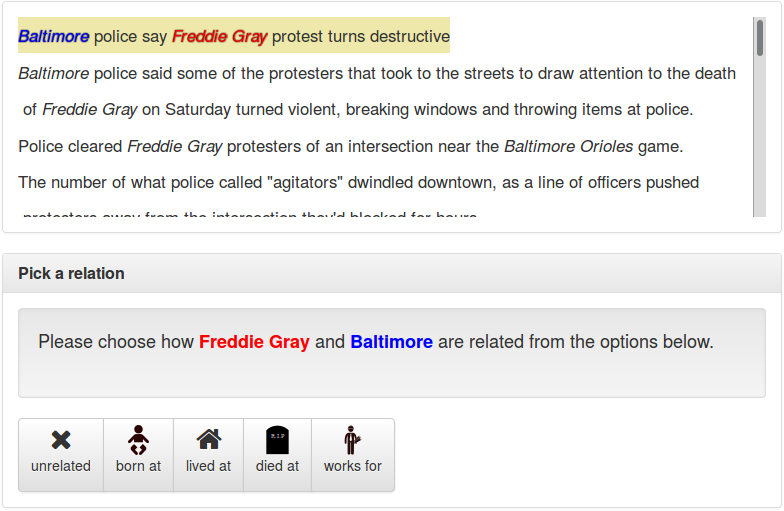
\includegraphics[width=\textwidth]{figures/interface/relation-interface}
    \caption{\label{fig:relation-interface}}
  \end{subfigure}
  \hfill
  \begin{subfigure}{0.49\textwidth}
  \centering
    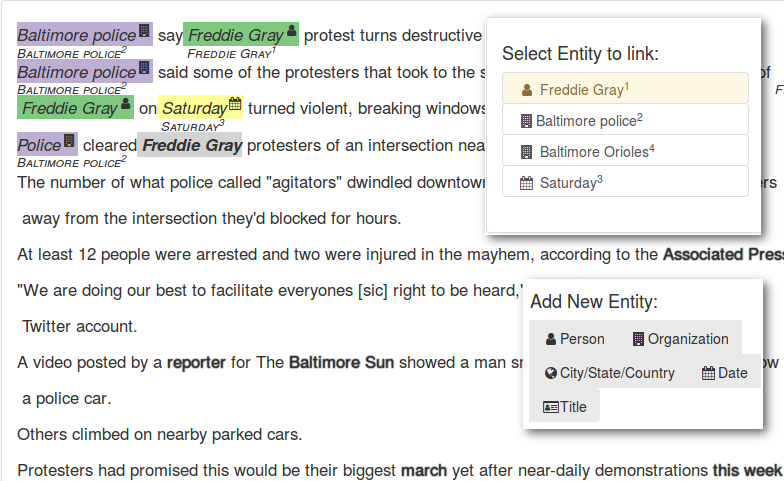
\includegraphics[width=\textwidth]{figures/interface/extraction-interface}
    \caption{\label{fig:entity-interface}}
  \end{subfigure} \\

  \begin{subfigure}{0.49\textwidth}
    \centering
    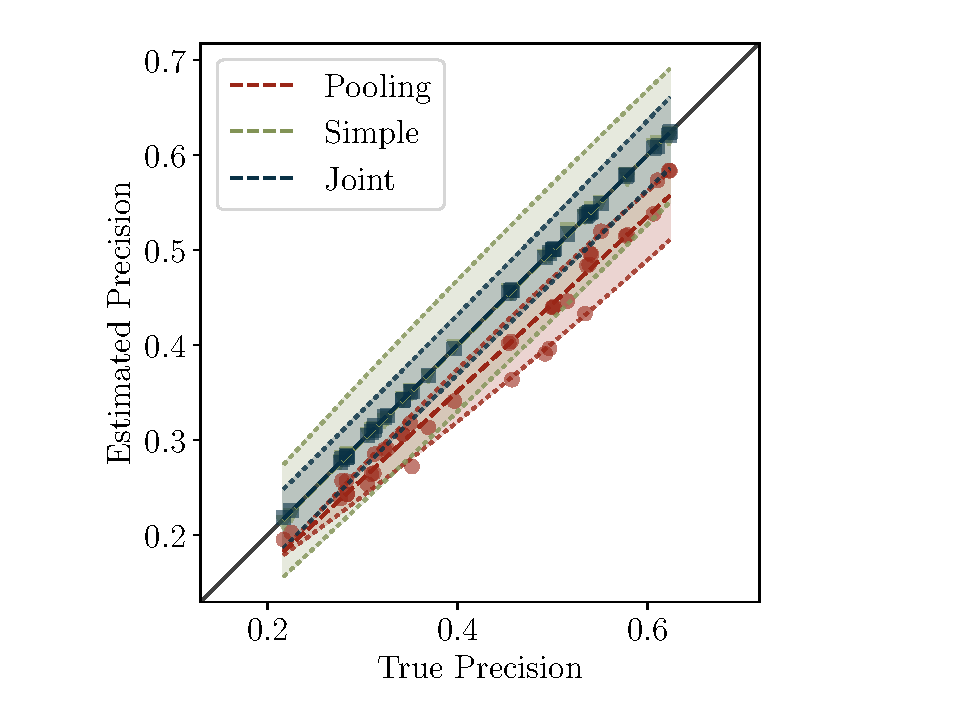
\includegraphics[width=\textwidth]{figures/simulation/simulation-p}
    \caption{}
  \end{subfigure}
  \hfill
  \begin{subfigure}{0.49\textwidth}
    \centering
    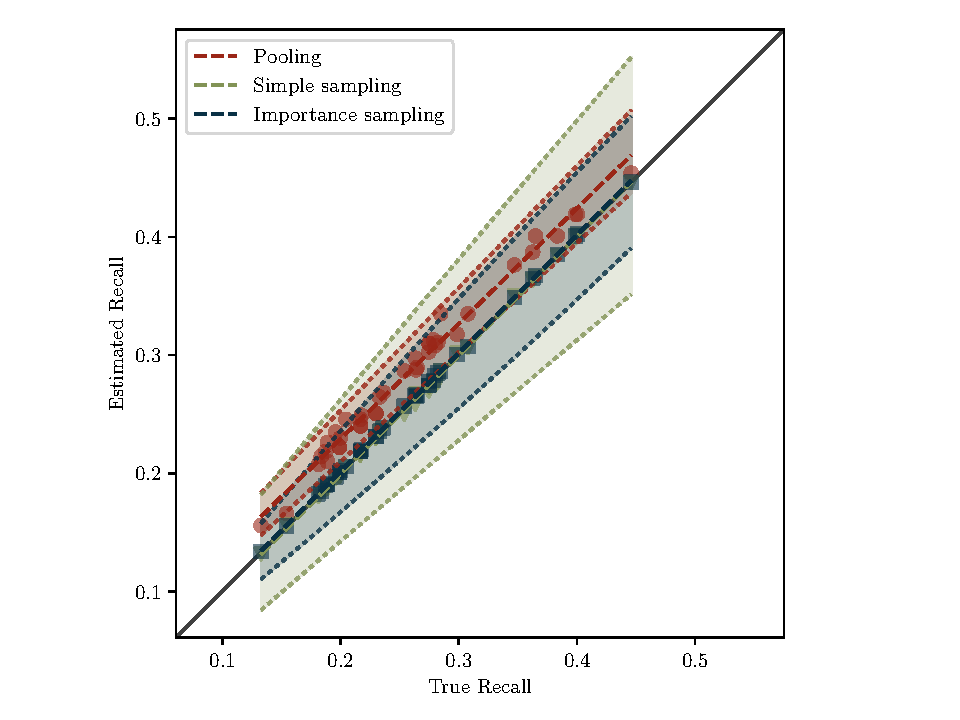
\includegraphics[width=\textwidth]{figures/simulation/simulation-r}
    \caption{}
  \end{subfigure} \\

  \begin{subfigure}{0.49\textwidth}
    \centering
    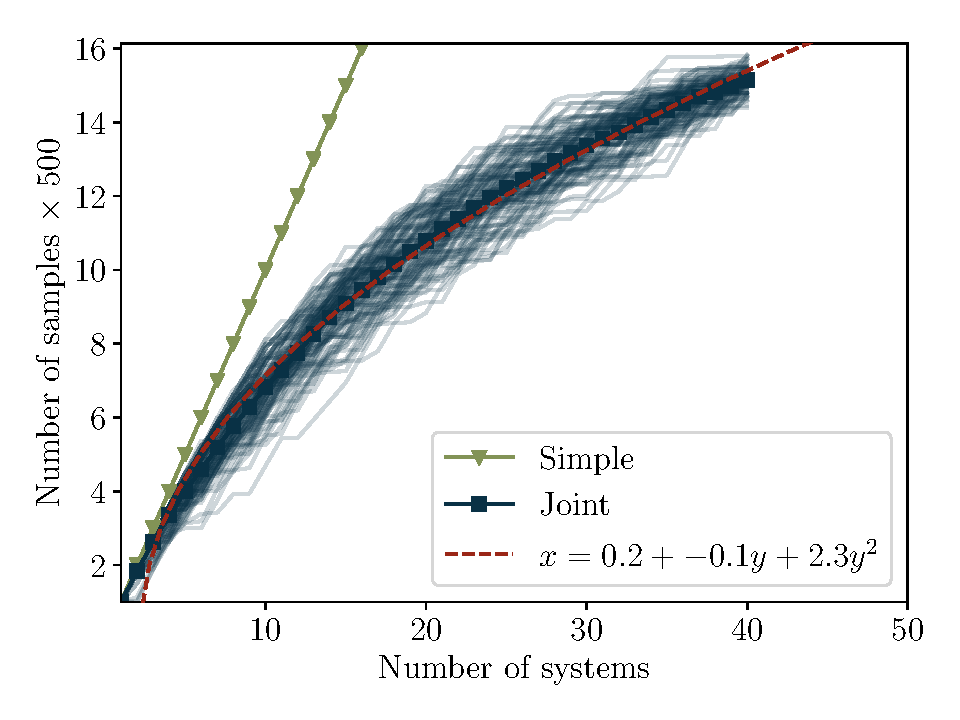
\includegraphics[width=\textwidth]{figures/simulation/simulation-n}
    \caption{}
  \end{subfigure}
  \hfill
  \begin{subfigure}{0.49\textwidth}
    \centering
    \section{Evaluation}
\label{sec:evaluation}

Let us now see how well on-demand open-world evaluation works in practice.
We begin by empirically studying the statistical properties of the proposed estimators by simulating the evaluation procedure on the TAC-KBP 2015 evaluation data and show that the estimators are indeed unbiased and that pooling does reduce variance.
We then show that the on-demand open-world evaluation methodology can serve as a practical replacement for the TAC-KBP competitions by actually running a mock evaluation TAC-KBP 2016 competition using our framework and showing that we obtain results of comparable quality at a fraction of the cost.

\subsection{Studying statistical properties with simulated experiments}
The statistical properties we'd like to study, namely bias and variance, require many repeated trials.
However, because the evaluation data in the TAC-KBP 2015 was collected by completely evaluating all predictions for 317 evaluation entities and 70 systems, we can simulate these trials by imagining that the evaluation data represents the universe of our output and treat a subset of the participating systems as submissions to our framework.

As baselines, we'll compare the precision and recall estimators proposed in \refsec{method} with the pooling-based methodology and with simple precision and recall estimators ($\pih^{(s)}$ and $\rhoh^{(s)}$) that do not reuse samples collected from other systems.
For the pooling-based methodology, we estimate bias and variance over many pool choices.
  On average, each pooled evaluation dataset has about \fake{1,000} evaluated instances.
For the sampling-based methodologies, we estimate bias and variance by running the experiment many times with about \fake{1,000} samples in total from all the different systems, making the two evaluation datasets comparable in terms of how many datapoints are drawn.

In \reffig{statistical-experiment}, we plot the precision and recall estimates made by each of these methods versus their ``true'' values which can be computed by looking at the entire evaluation corpus.
We see from the plots that the pooling-based methodology is significantly biased, while the sampling based estimators are not.
Furthermore, by incorporating samples drawn from other systems, the median variance reduces by a factor of \fake{4.1}, from \fake{0.2} (with the simple estimators) to \fake{0.05} (with the compound estimator).

\subsection{A mock evaluation for TAC-KBP 2016}
In \refsec{application}, we described the necessary elements required to apply on-demand open-world evaluation to KBP.
In particular, we needed to implement two crowd-worker interfaces to verify a relation tuple (i.e.\ evaluate $f(x)$) and to exhaustively annotate a document (i.e.\ to sample from $\sY$).
We have covered the cost and accuracy running these tasks in that section and will now study how well the evaluation framework works end to end. 

Using the algorithm described in \refalg{on-demand-sampling}, we evaluated three distinct relation extraction systems (a rule-based system, a supervised system and a neural network classifier) on 15,000 Newswire documents from 2016 TAC-KBP competition.
Each system uses Stanford CoreNLP~\citep{} to identify entities and the Illinois Wikifier~\citep{} to perform entity linking. 
In total, 100 documents were exhaustively annotated for about \$2,000, and 1000 of each systems submissions were annotated at about \$300 each, with 500 sampled to estimate macro-averaged relation scores and 500 were sampled to estimate macro-averaged entity scores.
\tableref{evaluation-results} presents the results of these systems on the mock evaluation.

\begin{table*}
  \centering
  \begin{tabular}{l l c c c} \toprule
    Scheme      & System    & $P^e (\pm 95\%)$ & $R^e (\pm 95\%)$ & $\fone{}^e (\pm 95\%)$ \\ \midrule
\multirow{3}{*}{Uncombined} &
  Patterns   & \fake{80.4 $\pm$ 3.0}\% & \fake{10.4 $\pm$ 5.0}\% & \fake{18.41 $\pm$ 4.3}\% \\
& Supervised & \fake{60.4 $\pm$ 3.0}\% & \fake{15.4 $\pm$ 5.0}\% & \fake{24.54 $\pm$ 4.3}\% \\
& Neural     & \fake{20.4 $\pm$ 3.0}\% & \fake{30.4 $\pm$ 5.0}\% & \fake{24.41 $\pm$ 4.3}\% \\ \midrule
\multirow{3}{*}{+ Pooling} &
  Patterns   & \fake{80.4 $\pm$ 3.0}\% & \fake{10.4 $\pm$ 3.0}\% & \fake{18.41 $\pm$ 3.0}\% \\
& Supervised & \fake{60.4 $\pm$ 3.0}\% & \fake{15.4 $\pm$ 3.0}\% & \fake{24.54 $\pm$ 3.0}\% \\
& Neural     & \fake{20.4 $\pm$ 2.6}\% & \fake{30.4 $\pm$ 2.7}\% & \fake{24.41 $\pm$ 2.6}\% \\ \bottomrule
  \end{tabular}
  \caption{\label{tbl:evaluation-results} Results from a mock evaluation.}
\end{table*}

%\footnote{A summary of mention-level scores \fake{can be found in the appendix}.}  
% How does cost compare?
% How do absolute scores compare?
Two immediate takeaways are that the precisions of these systems are \fake{on par with} the precisions reported as part of the official 2016 evaluation but the 95\% confidence interval is \fake{almost three times smaller}.
The recall scores on this evaluation are a significantly smaller than on the official 2016 evaluation.
Our explanation for this is that the exhaustive annotation required by our system is far more expansive and finds a lot of new entities that our mention detection systems. \fake{More error analysis.}

    %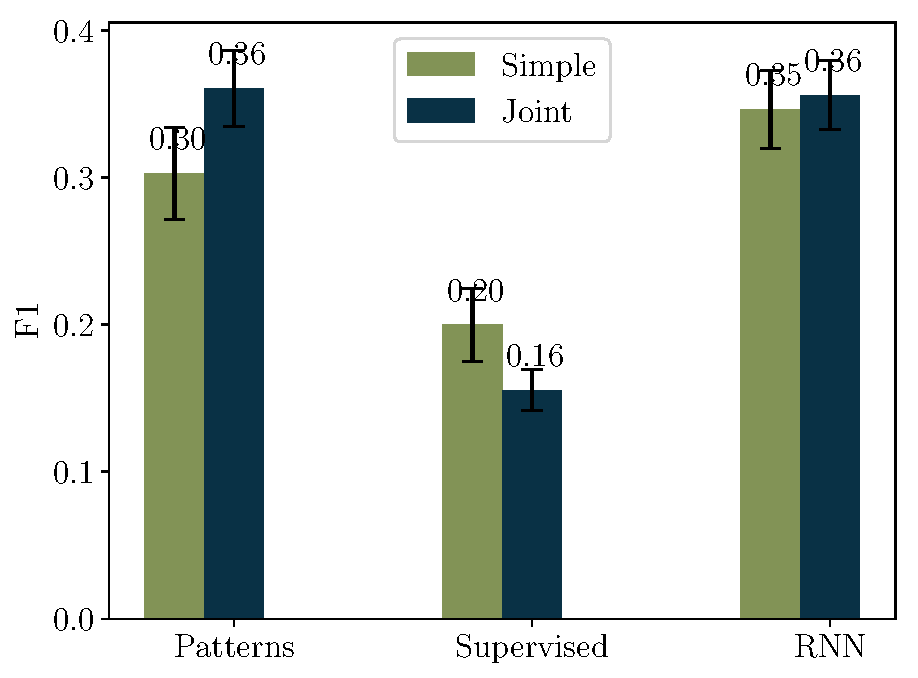
\includegraphics[width=\columnwidth]{figures/kbp2016/kbp2016_f1}
    \vfill
    \caption{\label{fig:evaluation-results}}
  \end{subfigure}

  \caption{\label{fig:simulation}
  \textbf{(a, b):} Interfaces for annotating relations and entities respectively.
  \textbf{(c, d):}
  A comparison of bias for the pooling, simple and joint estimators on the TAC KBP 2015 challenge.
  Each point in the figure is a mean of 500 repeated trials; dotted lines show the 90\% quartile.
  %The pooling based method uses between 5,000 and 6,000 labeled instances, while the sampling based methods use 
  %approximately 150 samples from each system.
  %Dashed trend lines indicate the mean bias of the estimation method: 
  %Unbiased estimates lie on the $y = x$ line.
  Both the simple and joint estimators are unbiased, and the joint estimator is able to significantly reduce variance.
  \textbf{(e):} 
  A comparison of the number of samples used to estimate scores under the fixed and adaptive sample selection scheme.
  %In the simulation, the top 40 systems were evaluated in randomized order to achieve a target variance equal to that obtained with 500 samples for a single system.
  Each faint line shows the number of samples used during a single trial, while solid lines show the mean over 100 trials.
  The dashed line shows a square-root relationship between the number of systems evaluated and the number of samples required.
  \ac{Note: fitting with a cubic gives $x = 0.01 y^3 -0.1y^2 + 1.8 y - 1.1$ with $R=1.0$.}
  Joint estimation combined with adaptive sample selection can reduce the number of labeled annotations required by an order of magnitude.
  \textbf{(f):} 
Precision ($P$), recall ($R$) and \fone{} scores from a pilot run of our evaluation service for ensembles of a rule-based system (R), a logistic classifier (L) and a neural network classifier (N) run on the TAC KBP 2016 document corpus. 
  }
\end{figure*}

\subsection{Sampling true instances}
Sampling from the set of true instances $\sY$ is difficult because we can't even enumerate the elements of $\sY$.
As a proxy, we assume that relations are identically distributed across documents and have crowdworkers annotate a random subset of documents for relations using an interface we developed (\reffig{entity-interface}).
Crowd workers begin by identifying every mention span in a document.
  For each mention, they are asked to identify its type, canonical mention within the document
  and associated Wikipedia page if possible.
They are then presented with a separate interface to label predicates between pairs of mentions within a sentence that were identified earlier.

We compare crowdsourced annotations against those of expert annotators using data from the TAC KBP 2015 EDL task on 10 randomly chosen documents.
We find that 3 crowdworkers together identify 92\% of the entity spans identified by expert annotators, while 7 crowdworkers together identify 96\%.
When using a token-level majority vote to identify entities, 3 crowdworkers identify about 78\% of the entity spans; this number does not change significantly with additional crowdworkers.
We also measure substantial token-level inter-annotator agreement using Fleiss' kappa for identifying typed mention spans ($\kappa = 0.83$), canonical mentions ($\kappa = 0.75$) and entity links ($\kappa = 0.75$) with just three workers.
Based on this analysis, we use token-level majority over 3 workers in subsequent experiments.
We also manually labeled 200 relation instances that from the exhaustively annotated documents and observed a precision of about 75\%.
While this precision is slightly less than the 80\% obtained by annotators at LDC \citep{ellis2016overview}, we believe it could be easily improved with appropriate changes to the annotation interface.
Consequently, we take a majority vote over 3 workers in subsequent experiments,
leading to a total cost of \$0.15 per relation instance.

The entity annotation interface is far more involved and takes on average about 13 minutes per document, corresponding to about \$2.60 per document, while the relation annotation interface takes on average about \$2.25 per document.
Because documents vary significantly in length and complexity, we set rewards for each document based on the number of tokens (.75c per token) and mention pairs (5c per pair) respectively.
With 3 workers per document, we paid about \$15 per document on average.
Each document contained an average 9.2 relations, resulting in a cost of about \$1.61 per relation instance.
We note that this is about ten times as much as labeling a relation instance.

We defer details regarding how documents themselves should be weighted to capture diverse entities that span documents to \refapp{implementation}.
%We provide details regarding our sampling scheme and its distribution over entities in \refapp{implementation} of the supplementary material.
%When considering uniformly sampled documents, we found that a majority of the relations extracted correspond to very rare entities and result in very few entities with more than one relation (\reffig{entity-distribution}).
%In contrast, the TAC KBP query are almost evenly split between rare and semi-frequent entities.
%As a heuristic, we adopt the following two-stage sampling procedure:
%First, 20\% of our exhaustive document collection is sampled uniformly and annotated.
%We then uniformly sample the entities annotated to create a collection of ``query entities''.
%Finally, we construct the remaining 80\% of our document collection by searching for documents that contain the query entities according to an exact string match. This process results in far more entities of medium frequency.
